\documentclass[11pt]{article}
\usepackage{enumitem}
\usepackage{latexsym}
\usepackage{amsfonts}
\usepackage{amsmath,amssymb,amsthm}
\usepackage{xcolor}

\usepackage{tikz}
\usetikzlibrary{arrows}
\usetikzlibrary{automata}

\setlength{\textheight}{8.5in}
\setlength{\textwidth}{6.0in}
\setlength{\headheight}{0in}
\addtolength{\topmargin}{-.5in}
\addtolength{\oddsidemargin}{-.5in}

\input{preamble.tex}

\newcommand{\bl}[1]{\textcolor{blue}{#1}}
\newcommand{\rd}[1]{\textcolor{red}{#1}}

\begin{document}
\hw{2: Nondeterminism and Pumping Lemma}{01/22/2026}{}{Due:02/05/2026}

This assignment is due on \textbf{11:59 PM EST, Thursday, February 05, 2026}. You may turn it in up to 48 hours late, but assignments turned in by the deadline receive 3\% extra credit.  Additionally, late submission means late feedback, which means less time to study before an exam.

You should submit a typeset or \emph{neatly} written pdf on Gradescope. The grading TA should not have to struggle to read what you've written; if your handwriting is hard to decipher, you will be asked to typeset your future assignments. 

Enter your work using the \verb|answer| environment we have provided for you. The default color is \textcolor{teal}{teal}, but you can choose to change it to any of \rd{red}, \textcolor{brown}{brown}, \textcolor{magenta}{magenta}, \textcolor{violet}{violet}, \textcolor{blue}{blue}, \textcolor{darkgray}{darkgray}, or black like so:
\begin{verbatim}
                        \begin{answer}[<COLOR>]
                            <YOUR WORK GOES HERE> 
                        \end{answer}
\end{verbatim}

You may collaborate with other students, but any written work should be your own. 

\begin{enumerate}
    \item \textbf{Nondeterminism} (4 points) \\
    For the following proofs, you must provide a construction of a finite automaton by describing its components to show that the language is regular. \\
    
    (2 points - \textit{Section A}) For any regular language $L$, prove that $L' = $ $\{w\ \text{where all a's are removed} |\ w \in L, a \in \Sigma\}$ is regular.
    
    \begin{answer}
        % Enter your solution here!
    \end{answer}
    
    (2 points - \textit{Both}) 
    For any regular language $L$, prove that $L' = $ $\{xay\ |\ xy \in L, a \in \Sigma, x, y \in \Sigma^*\}$ is regular. Notice that we form $L'$ by taking the strings in $L$, and adding a single symbol anywhere in the string, even possibly at the beginning or end. 
    
    \begin{answer}

        First let us denote the addition symbol as $\alpha \in \Sigma$. Now if $L$ is regular then there exists some DFA that accepts it. Now every DFA is an NFA, so let's consider this to be some NFA, $N$, that accepts $L$. Now we make the following modification:
        \begin{enumerate}
    \item In our new NFA labeled $M$, we create two copies of $N$. If $r_i$ denote the states of $N$, then $p_i$ and $q_i$ denote the new copies corresponding to $r_i$ such that if $\delta$ is our new transition function and $\delta_0$ was that of $N$, then we have $\delta(q_i, k) = \delta_0(r_i, k)$ and $\delta(p_i, k) = \delta_0(r_i, k)$. We also make sure to unmark the start and accept states in $M$ except for that in $p$ (i.e., if $r_k$ is an accept state in $N$, then we unmark $q_k$ as an accept state but $p_k$ will still be an accept state).
    
    \item We now add a new start state $q_{\alpha}$ such that $\delta(q_{\alpha}, \epsilon) = q_1$ and $\delta(q_{\alpha}, \alpha) = p_1$ for all $\alpha \in \Sigma$.


\item Now for each $q_i$ we have $\delta(q_i, \alpha) = p_i$ for every $\alpha \in \Sigma$.

\begin{figure}[h]
  \centering
  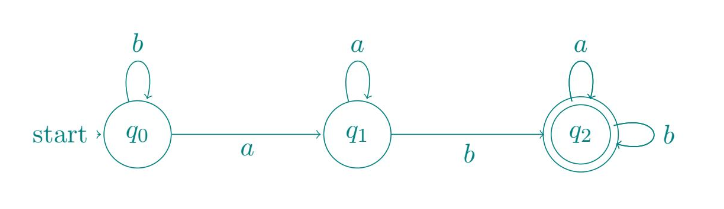
\includegraphics[width=0.8\textwidth]{assets/d1.png}
  \label{fig:d1}
\end{figure}
In this case the modification we make is as follows,

\begin{figure}[h]
  \centering
  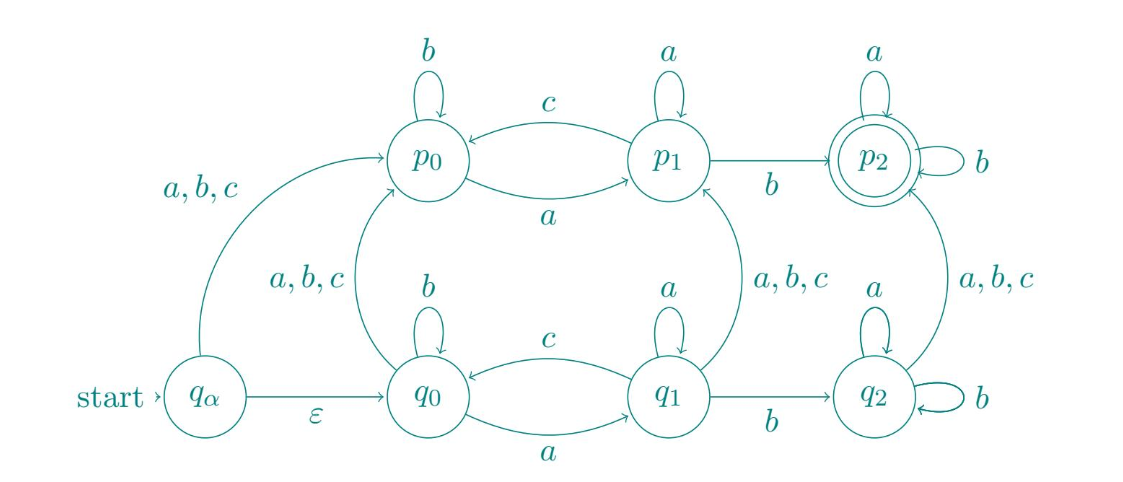
\includegraphics[width=0.8\textwidth]{assets/d2.png}
  \label{fig:d2}
\end{figure}

Now we need to show that $M$ accepts all strings in $\{xy : xy \in L, \, x, y \in \Sigma^*\}$. Consider two arbitrary strings $x, y \in \Sigma^*$ such that $xy \in L$. And take an arbitrary symbol $\alpha \in \Sigma$. Now note that as $x \in L$ the $q$ states will simulate $x$ as in the original DFA. Now given the symbol $\alpha$, the NFA can choose to transition to the corresponding state in $p$, now as the states $p$ are also a perfect simulation of the original DFA the string $y$ will also be accepted. Hence, we show that any string of the form $x\alpha y$ such that $xy \in L, \, \alpha \in \Sigma, \, x,y \in \Sigma^*$ is accepted by $M$. On the other hand consider a string that is accepted by our automate. Now for a string to be accepted it needs to jump to the $p$ states from the $q$ states. Let a string before the jump be $x$, let the jump be $\alpha$  and let the string after the jump be $y$. Now note that if $x$ ends at $q_n$ then $y$ begins at $p_n$ as per our construction. But as the $p$ states are a simulation of our original DFA, this means that we have $xy$ a string that is accepted by the original DFA and hence we can write any string in the form $x \alpha y$ where $xy \in L$ and $\alpha$ some alphabet.
    
\end{ins }

\end{enumerate}
    \end{answer} 
    
    (2 points - \textit{Section X}) Let $L$ be a regular language, and let $L^\#$ be the set $\{x \in \Sigma^*\ |\ \text{for some } y \in L, y \text{ has the same number of } 1\text{'s as x}\}$. Prove that, if $L$ is regular, $L^\#$ is regular.
    
    \begin{answer}
    If $L$ is regular, there is a DFA for it, and consider this to be the NFA of $L$ called $N$. Now for each state $q \in Q$ of $N$, we modify $\delta$ such that $\delta(q, a) = q$ where $a \in \Sigma$ and $a \neq 1$ and for any $a$ such that $\delta(q_0, a) = q_1$ where $q_0 \neq q_1$ we add $\delta(q_0, \epsilon) = q_1$. The point of these two additions is that we allow each state to loop to itself any number of times as long as it’s not a 1, as we only care about the counts of 1’s. And the second modification allows us to skip transitions that are not 1 as again we don’t want to enforce the other structures of $L$ that do not count the 1.

    Now assume that $x$ is a string accepted by our new NFA. Now running down the computation for this string, at each state we have three choices. To self loop an alphabet other than 1, to $\epsilon$ transition (if it exists) or to take the transition like that of the original DFA. Now the first two options do not add or remove from the number of 1's (note that although it’s possible for us to have an $\epsilon$ and 1 transition, the $\epsilon$ transition implies that in the original DFA it was also possible to skip the 1), so the third option would be to follow the transition of $L$ in which case we preserve the count of 1. So we show the computation preserves the count of 1 to that of $L$ and hence the string is in $L^{\#}$.

    Now assume $x \in L^{\#}$ we need to show that $x$ is a string accepted by our NFA. Now clearly $x$ has the same number of 1’s as in some string $y \in L$ (by definition of $L^{\#}$). Now this means that by adding or removing non-1’s from $y$ we can construct $x$. Let $y_0 \cdots y_n$ be our string, then after each $y_i$ we can either add non-1’s or for each $y_i \neq 1$ we can replace it with $\epsilon$. So first note that $y$ is trivially accepted by our NFA as we preserve the DFA of $L$. So for each $y_i$ our new NFA is in some state $q_i$, now addition of non-1 states is allowed as we allow self loops for non-1’s, and removal of $y_i \neq 1$ is allowed by allowing $q_i$ to skip to $q_{i+1}$. Hence, our NFA is able to simulate any function that transforms $y \in L$ to $x \in L^{\#}$ and hence we have $x \in L^{\#}$.


    \end{answer}
    
    \newline

    \item \textbf{Regular Expressions} \textit{**Both Sections**}(4 points) \\ 
    For the following parts, you may assume $\Sigma = \{0, 1\}$. 

    (2 points) Give a regular expression for each of the following languages: 

    \begin{itemize}
        \item The set of all strings with a multiple of three number of ones.
        
        \begin{answer}

            $0^{*}(10^{*}10^{*}10^{*})^{*}$
        \end{answer}
        
        % \item The set of all even length strings with at most two 0's 
        \item The set of all strings where the number of 0's is equivalent to $2\ mod\ 3$. 
        
        \begin{answer}

            $1^{*}01^{*}0 (01^{*}01^{*}0 | 1)^{*}$
        \end{answer}
        
    \end{itemize}

    (2 points) Give an equivalent NFA for the following regular expression:
    
    $((11 \cup 01^*1 \cup 01)0)^*(11)^*$

    \begin{answer}
        \begin{center}
      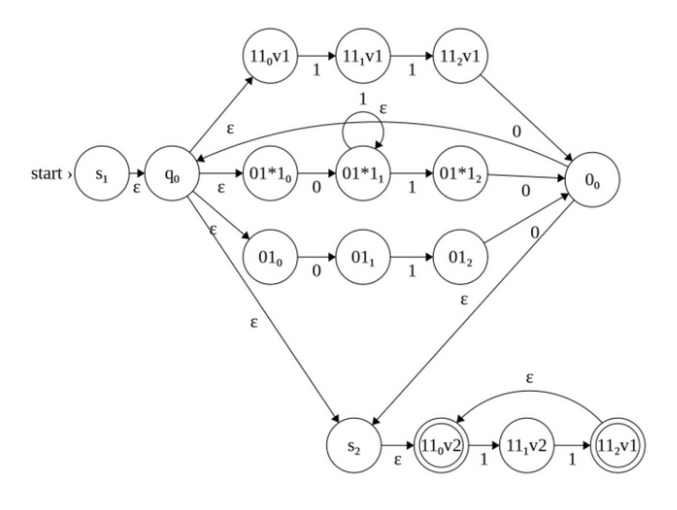
\includegraphics[width=0.8\textwidth]{assets/nfa.png}
        \end{center}
    \end{answer}
    
    
    \item \textbf{Pumping Lemma} (4 points) 

    (\textit{Section A}) Prove that $L_1 = \{a^ib^j\ |\ |i-j|$ is prime$\}$ is not regular.
    
    \begin{answer}
        % Enter your solution here!
    \end{answer}
    
    
    (\textit{Section X}) Prove that $L_2 = \{a^ib^j\ |\ i,j$ are relatively prime$\}$ is not regular. 
    
    \begin{answer}
        % Enter your solution here!
        We have $a^i b^j$ where $i, j$ are coprime. Assume that the language is regular with pumping length $p$. So consider the string $a^q b^{q+1}$ where $q$ is a prime number greater than $p$, this can be written as $s = xyz$ where for any $i > 0$ we have $x y^i z$ a element of our language. Now note we have three options for $y$,

\begin{enumerate}
    \item[a)] $y$ contains both $a, b$. In this case note that we would end up with $a$'s and $b$'s interleaved and hence would not be in our language.
    
    \item[b)] $y$ consists of only $a$'s. Note that we have the condition that $|xz| \leq p$, but if $y$ consists of only $a$'s and because $z = b^{q+1}$ and $q+1 > p$ we have it that $|xz| > p$, a contradiction.
    
    \item[c)] So the only option is if $y$ consists of only $b$'s. Note that in this case we have $a^q b^k b^l$ such that $k + l = q + 1$. Now note that if we have $y^i$ for any $i$ then we have $ki + l$ $b$'s. However, notice in the equation $ki \equiv -l \ (\text{mod} \ q)$ as $q$ is prime this means that $(k, q) = 1$ and hence $k$ has an inverse modulo $q$. Hence, we have $i \equiv -lk^{-1} \ (\text{mod} \ q)$ an equivalently an $i$ such that $q | ki + l$ or $(q, ki + l) > 1$. But this implies that our string $x y^i z$ is NOT a string in our language as the powers of $a$ and $b$ share a common factor, namely $q$ in this case. A contradiction. Hence this case also doesn't work.
\end{enumerate}

    \end{answer}
    
    
    \item [4.] \textbf{Pumping Lemma Adjacent} \textit{**Section A only**} (4 points)

    A \emph{minimal} DFA $D$ for a language $L$ is a $DFA$ such that any DFA for $L$ has at least as many states as $D$.  Complete the steps below to prove the following claim:
    \newline

    \emph{Claim:} For any positive integer $n \geq 3$, there is a language whose minimal DFA contains $n$ states.
    \newline

    \emph{Proof:} For some $k \in \mathbb{Z}$, let $L_k = \{a^k\}$, a set with one element. Now, suppose $D$ is a minimal DFA for $L_k$. You will prove that $D$ has at least $k+2$ states.  Let $\{q_i\}_{i=0}^k = q_0, …, q_k$ be the sequence of states (not necessarily distinct!) that $D$ follows when reading $a^k$. 
    \newline

    (1 point) Explain why $\{q_i\}_{i=0}^k$ cannot contain any repeated states (hint: the proof of the pumping lemma), and conclude that $D$ has at least $k+1$ states.
    
    \begin{answer}
        % Enter your solution here!
    \end{answer}
    
    \newline

    (1 point) Now consider the state that $D$ ends in upon reading the string $a^{k+1}$, and argue that $D$ must have at least $k+2$ states.
    
    \begin{answer}
        % Enter your solution here!
    \end{answer}
    
    \newline

    (1 point) Demonstrate that $D$ has exactly $k+2$ states by giving an explicit construction of $D$.
    
    \begin{answer}
        % Enter your solution here!
    \end{answer}
    
    \newline

    (1 point) Complete the conclusion of this proof: ``Therefore, we have given a constructive proof of the original claim. For any $n \in \mathbb{Z}, n \geq 3$, the language \_\_\_\_\_\_\_\_\_\_ has a minimal DFA with $n$ states."

    \emph{Hint: Your answer should be something, like $L_{3n}$, in terms of n.}
    
    \begin{answer}
        % Enter your solution here!
    \end{answer}
    
    \newline

    \item [5.] \textbf{Polynomial Length} \textit{**Section X only**} (4 points)\\
    Given $f(n)$, a polynomial with non-negative integral coefficients, let $L_f = \{1^{f(n)} ~|~ n \in \mathbb{N}\}$.
    \begin{itemize}
        \item For exactly which $f(n)$ is $L_f$ regular? Prove your answer. 
        
        \begin{answer}
            % Enter your solution here!
            We know that our alphabet consists of just 1's and that we have a finite automata. First let’s analyze all the possible automata that we can make under these conditions. As we only have one alphabet, each state has only one arrow going away from it or towards it. So we have two cases,

\begin{enumerate}
    \item[a)] We have no true loops in our automata. In this case this we have no loops at all (so no self loops either). But in this case the range i.e the language that is accepted in finite. Now note that given a polynomial with positive integral coefficients, if the coefficients of $n^{k}, k \ge 1$  are non-zero then $f$ is increasing and hence has a countable range. So the only option is that all those coefficients are zero and our function is $f(n) = k$ where $k \in \N$.
    
    \item[b)] Second case is we have only ONE loop. Note that we CANNOT have more than one loop. Assume we have two loops for instance, then there must exist a state that has two transitions for the same alphabet (in this case 1) as we would need one to continue a loop and one to get one of the first loop. However, if we only have ONE loop, we do not need a transition to escape the loop.
    \vspace{1em}

        
\end{enumerate}

    Now this could either be a self loop or a loop with more than 1 state. In both cases consider the two divisions in the DFA, a finite length of states and a finite loop. With the finite length of states we can only have a finite range (and note we showed above this can only be generated by a constant) and the loop (say the loop is length $k$) will generate values of the form $a_{0} + kn$ where $a_{0}$ is some constant number of states we have to pass through before reaching the loop. So the possible functions are of the form $a_{0} + a_{1}n$ where $n \ge 0$. So we've shown that all the DFAs will generate  either of these two functions which means that any other polynomial that have non-zero coefficients for $n^2, \dots$ cannot form a regular language as we did above.
    

        \end{answer}
        \item Prove that for all other $f(n)$, $L_f$ is not regular.

        \begin{answer}
            % Enter your solution here!
            Clearly we showed above the every DFA that can be formed can be mapped onto a function of the form we described above. The contrapositive of this statement implies that for every function not of that form there does not exist a DFA that accepts it and hence is not regular.

            \vspace{1em}
            Or another way of looking at it is, assume a polynomial $f$  that is not linear in $n$ is such that $1^{f}$ is a regular language i.e has a DFA. Now using the pumping lemma let $p$ be the pumping length and let $w$ be some string greater than the pumping  length. We write $w = xyz$ where $|y| \ge 1$ and $|xz| < p$. Note now that any string of the form $xy^{i}z$ is accepted by the language. Let $|y| = k$ this must then mean that if $|w| = h$ then the strings $1^{h}, 1^{h + k}, 1^{h + 2k}, \dots$ are all accepted by the DFA. But note now that if $f$ is non-linear then it cannot produce numbers of the form $h, h + k, h + 2k, h + 3k, \dots$ as $f$ must increasing exponentially or in other words if $n > m$ then $f(n + 1) - f(n) > f(m + 1) - f(m)$ (note it's strictly greater). But this is a contradiction as we just showed that we have a difference of $k$ for each of the values.
        \end{answer}
    \end{itemize}
\end{enumerate}
\end{document}
